\subsection{User Interface Design}
When designing an interface, the purpose of the service comes into question. It is important to define what drives each page of the application, and what the core functionality of it is in order to choose the best layout and color scheme for the component\textquotesingle s representation and the user\textquotesingle s accessibility. In addition, identifying the core user base is also important in designing the interface.

\subsubsection{Interface Color Selection}
For this service, some pages are visually driven, with little text on the screen, while some are text driven. The Analysis section of the Catalog for instance relies on the data visualization component as the main focal point, while the Job Creation page is focused on taking the user though logical steps to create jobs and manage input files.\par
When selecting a color palette, we took inspiration from our sponsor\textquotesingle s logo made for his research that contains core colors of gold (#b6cd26) and black. We liked this logo from the get go and wanted to incorporate these colors into the application. To go along with the nature focused theme of our project, we added a green color (#4d9574) that went well with the gold. We decided to used black for the nav bar, which will contrast with gold. White is used as the main background to give the app a clean and simple look. Important content contained in Material-UI Paper components, which are styled with a box shadow, so that their content stands out against the white background. All buttons in our app are a gradient of gold and green.\par
With pages that are mainly visually driven, like the Analysis tab of the Catalog page, it is important for the data visualizations to stand out. Contrast in pages is important for drawing attention to elements and directing the user\textquotesingle s eyes. To stand out against the white background of Mangrove, we decided to have bright colors in our graphs. With multiple colors being used in graphs to represent results of different jobs.\par
The colors used in the Job Creation page and the selection tabs of the Catalog are kept simple, too allow users to focus on creating and selecting jobs. Green is used in checkboxes and blue is used for the stepper icons and radio buttons. The Job Queue page uses different colors for each job status, so users can easily tell if a job is in progress, completed or has failed.\par

\subsubsection{Page Organization}
Page organization is important for putting elements in a logical and meaningful place. Placing related content together helps the end user be more efficient, especially on pages like the Job Creation page. The following thought process went into each page.\par
The Job Creation page is where users will upload files, as well as define and start jobs on their sets of sound files. Based on input from our sponsor, this is the first page a user will see after logging in. The organization of this page is based on the step by step process of starting jobs. A Material-UI Stepper component is used, with the next button being disabled until all required information of that step is given. When a user first visits this page, they will be taken to step one, choosing files for a new set of jobs. They will see a table of all sound files that have already been uploaded in a tab. A second tab will bring the user to a component to upload more files. Users can use a feature to automatically import information like recording time if it is contained in the file names. If the user does not have a set naming convention, text boxes and date pickers are provided to fill in this information in the upload table. After files have been selected, the next button will be clickable and they can move on to choosing the index. This step includes radio button for each index, with some information from the R Soundecology package. The last step is defining specs. A table will be shown with all previously used specs and input fields for new specs, with a checkbox to use default specs. The user can then click Finish and the jobs will start processing.\par
The Job Queue page shows user the progress of jobs currently running. This page makes requests to get the status of running jobs in a timed interval. Users will be able to see when each job finishes processing and can clear completed jobs from the table.\par 
The Catalog page contains the user\textquotesingle s results from past jobs and allows them to filter through them and view the Analysis for whichever they\textquotesingle d like. This page includes tabs for each step involved in selecting jobs and a tab for viewing visualizations. The first three tabs let the user filter specs, inputs and jobs and then select the ones to be analysed from a table to the right of the input text fields. The Analysis tab first has the user select sets of jobs to compare and then provides all available graphs for the index used on those jobs in expansion panels. The use of expansion panels lets users focus on the graphs that are relevant to their current research. Points of the graphs can be clicked on to show an audio player, which starts at the time in the files corresponding to the data point clicked. This audio player will scroll with the page so other graphs can be viewed while listening. For each file set, a button to download data to a CSV is shown. This opens a modal that lets the user select which information should be exported.\par

\subsubsection{Page Use Cases}
\begin{center}
  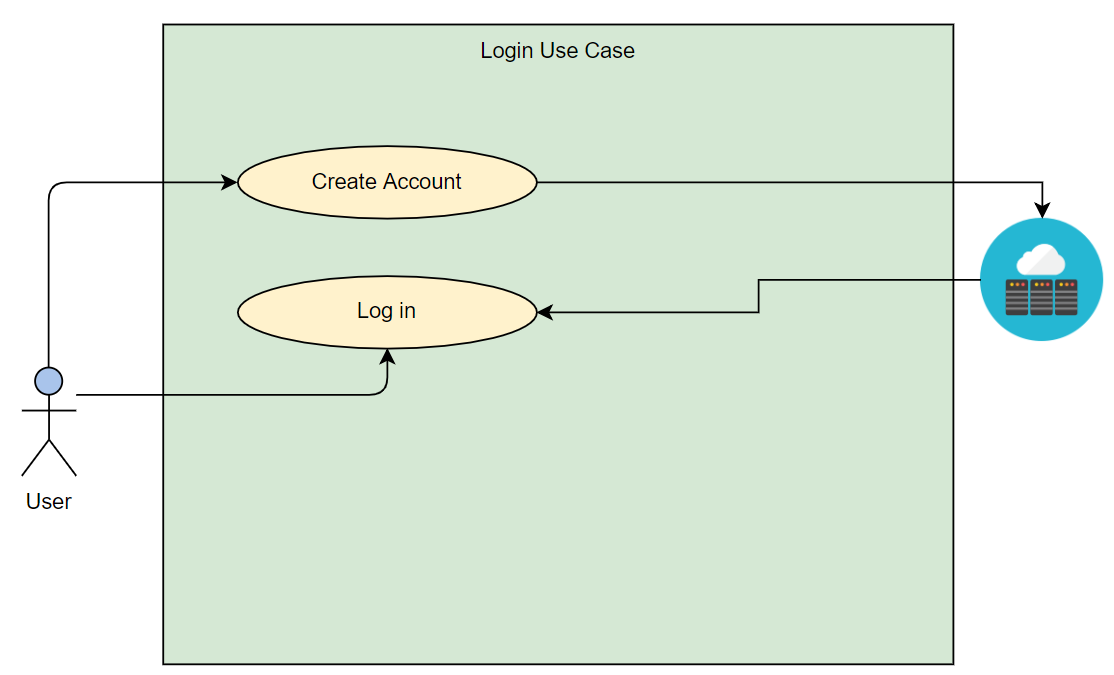
\includegraphics[width=\textwidth]{UseCaseLogin} \\[12pt]
\end{center}
\begin{center}
  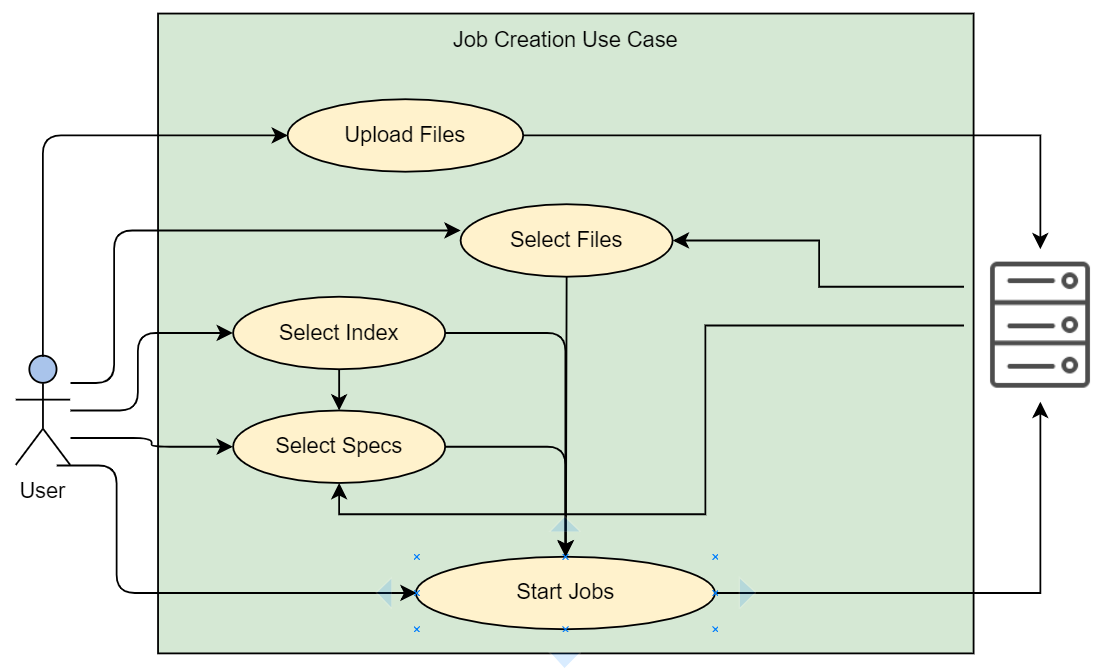
\includegraphics[width=\textwidth]{UseCaseJobCreation} \\[12pt]
\end{center}
\begin{center}
  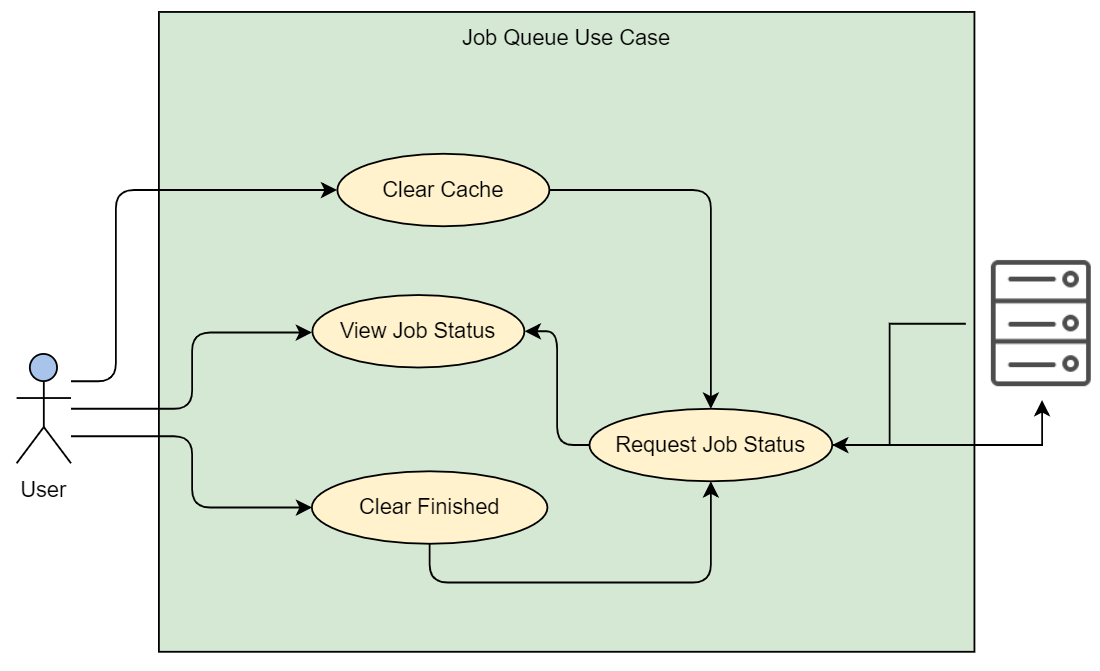
\includegraphics[width=0.85\textwidth]{UseCaseJobQueue} \\[12pt]
\end{center}
\begin{center}
  \includegraphics[width=\textwidth]{UseCaseCatalog} \\[12pt]
\end{center}
\begin{center}
  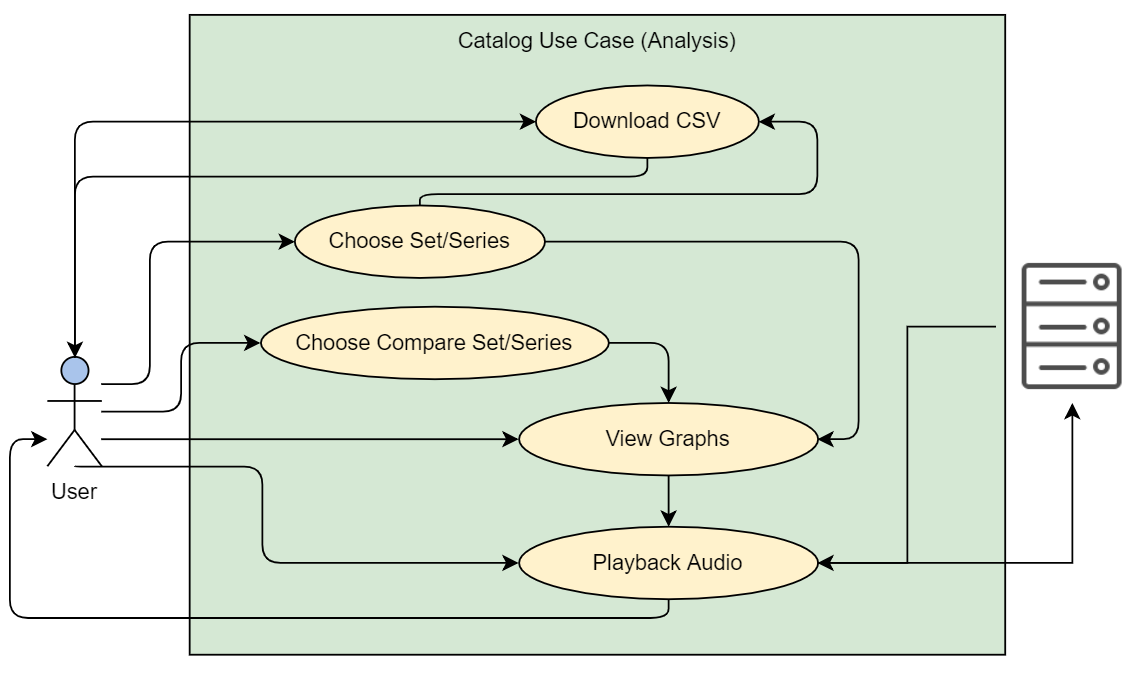
\includegraphics[width=\textwidth]{UseCaseAnalysis} \\[12pt]
\end{center}

\subsubsection{Frontend Frameworks}
A big part of getting the front end of the service up and running as quickly as we did was the use of frameworks. The core frameworks for this project are explained in the Infrastructure section of this project, so this will only cover the core frontend frameworks. The core frameworks used are as follows:
\begin{itemize}
  \item Material-UI
  \item Bootstrap
  \item Recharts
\end{itemize}
Material-UI is a framework for React that includes new components to easily add into the existing pages, handling styling for these components to help save time in development. This framework is used heavily in both the Catalog and Job Creation pages.\par
Bootstrap is a CSS framework made to handle screen size changes without hassle on the developer\textquotesingle s end. Bootstrap divides the page up into twelve parts, containing rows and columns. Components can then be placed into their respective rows and columns, including nesting, to create a functional and dynamic interface. This framework is especially useful for us to handle changing screen sizes.\par
For the Analysis part of the Catalog page, we needed a framework to turn our JSON data into graphics based on the user selected result from the result table. Recharts is a framework for doing just that, and is in charge of creating the respective data visualizations for each index. Recharts provides easy to use code made specifically for React to turn our data into nice, concise graphics.
